% !TEX TS-program = pdflatex
% !TEX encoding = UTF-8 Unicode

% Personalización de la clase `scrartcl` del paquete KOMA-script
% para incluir márgenes amplios
% Francisco Torralbo Torralbo
% 2019-02-28

\documentclass{scrartcl} 

\KOMAoptions{%
  twoside,
  fontsize=10pt,
  paper=a4,
  parskip=half,
  headsepline,
  toc=bibliography,
  toc=indent,
  DIV=9,            % Cambia el ancho del texto
  mpinclude=true,   % Incluimos el margen en el cálculo del diseño
  BCOR=0mm          % No reserva espacio de margen para encuadernación
}

% Finalmente el siguiente comando controla el ancho del margen.
\setlength{\marginparwidth}{1.5in}

% Idioma y codificación
\usepackage[activeacute,spanish]{babel}
\usepackage[utf8]{inputenc}
\selectlanguage{spanish}

% Tipografía
\usepackage[sc, osf]{mathpazo} % Tipo de fuente
\usepackage[activate={true,nocompatibility},final,tracking=true,kerning=true,spacing=true,factor=1100,stretch=10,shrink=10]{microtype}

% Tablas, gráficos y color
\usepackage{booktabs}
\renewcommand{\arraystretch}{1.5} % Aumenta el espacio vertical entre las filas de un entorno tabular

\usepackage{graphicx}
  % path to the graphics folder
  \graphicspath{{img/}}

\usepackage{color}
  \definecolor{darkgray}{gray}{0.3} % Color que se usará para las notas al margen

% Cabeceras: personalización de la cabecera con el paquete `scrpage2`
\usepackage[headsepline]{scrlayer-scrpage}

  % Los siguientes comandos cambian el color y tipo de letra de la cabecera.
  \setkomafont{pageheadfoot}{\color[rgb]{0.4,0.4,0.4}\scshape\sffamily}
  \addtokomafont{headsepline}{\color[rgb]{0.4,0.4,0.4}}
  \setkomafont{pagenumber}{\color[rgb]{0.4,0.4,0.4}\sffamily}
  \addtokomafont{footsepline}{\color[rgb]{0.4,0.4,0.4}} 

  % Lo siguiente define qué incluir en la cabecera y pie así como dibujar una línea en la cabecera que cubra el margen
  \pagestyle{scrheadings}
    \clearscrheadfoot
    \ihead{\headmark}
    \ohead{\pagemark}
    \setheadwidth[0pt]{textwithmarginpar}
    \setfootwidth[0pt]{head}

% Peronalización para incluir notas al margen

 \usepackage{ifthen}
\usepackage{calc}

% Los siguientes tres paquetes son para poner correctamente notas al margen con el comando \sidenote y \marginnote.
\usepackage{sidenotes, mparhack, ragged2e}
  % Las definiciones siguientes permiten cambiar el tipo de letra y color de las notas al margen
  \let\oldmarginpar\marginpar
  \renewcommand\marginpar[1]{\-\oldmarginpar[{\RaggedLeft\footnotesize\sffamily \textcolor{darkgray}{#1}}]%
  {\RaggedRight\footnotesize\sffamily \textcolor{darkgray}{#1}}}
  \let\oldmarginnote\marginnote
  \renewcommand\marginnote[1]{\-\oldmarginnote[{\RaggedLeft\footnotesize\sffamily \textcolor{darkgray}{#1}}]%
  {\RaggedRight\footnotesize\sffamily \textcolor{darkgray}{#1}}}

% Definición del entorno `fullwidth`

\newlength{\overhang}
\setlength{\overhang}{\marginparwidth}
\addtolength{\overhang}{\marginparsep}

\newlength{\fullwidthvalue}
\setlength{\fullwidthvalue}{\textwidth}
\addtolength{\fullwidthvalue}{\overhang}

%
\newenvironment{fullwidth}
  {\ifthenelse{\boolean{@twoside}}%
     {\begin{adjustwidth*}{}{-\overhang}}%
     {\begin{adjustwidth}{}{-\overhang}}%
  }%
  {\ifthenelse{\boolean{@twoside}}%
    {\end{adjustwidth*}}%
    {\end{adjustwidth}}%
  }

% ---- HYPERREF -------------------------------------------
\usepackage[unicode,psdextra]{hyperref}
\hypersetup{
  %colorlinks,
  pdftitle={},%
  pdfauthor={},%
  pdfkeywords={},%
  pdfcreator={pdfLaTeX},%
  pdfproducer={LaTeX with hyperref},
  urlcolor=[rgb]{0.2,0.1,0.5},
  linkcolor=[rgb]{0.2,0.2,0.2},
  citecolor=[rgb]{0.2,0.2,0.2}
}

% Información del documento
% \titlehead{}         
\subject{Curso LaTeX}
\title{Título}
\author{\href{http://www.ugr.es/local/ftorralbo/}{Francisco Torralbo}}
%\date{}

\begin{document}

\maketitle

\begin{abstract}
Lorem ipsum dolor sit amet, consectetur adipisicing elit, sed do eiusmod tempor incididunt ut labore et dolore magna aliqua. Ut enim ad minim veniam, quis nostrud exercitation ullamco laboris nisi ut aliquip ex ea commodo consequat. 
\end{abstract}

\section{Plantilla}
Lorem ipsum dolor sit amet, consectetur adipisicing elit, sed do eiusmod tempor incididunt ut labore et dolore magna aliqua. Ut enim ad minim veniam, quis nostrud exercitation ullamco laboris nisi ut aliquip ex ea commodo consequat. 

\begin{marginfigure}%
  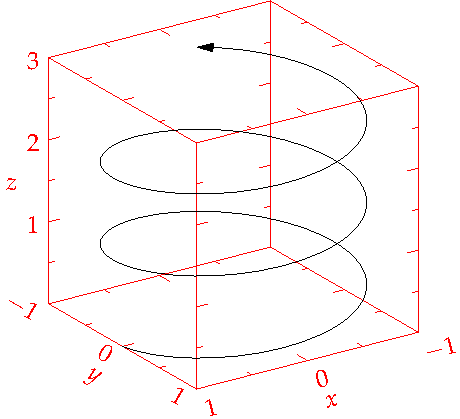
\includegraphics[width=\linewidth]{helix}
  \caption{Esta es una figura al margen incluida con el entorno \texttt{marginfigure}.}
  \label{fig:marginfig}
\end{marginfigure}

\subsection{Notas al margen}\label{sec:sidenotes}

Puedes incluir notas al margen con el comando \verb|\sidenote|\sidenote{Esta nota al margen ha sido incluida con el comando \texttt{\textbackslash sidenote}.}, consectetur adipisicing elit, sed do eiusmod tempor incididunt ut labore et dolore magna aliqua. Ut enim ad minim veniam, quis nostrud exercitation ullamco laboris nisi ut aliquip ex ea commodo consequat. 

También puedes incluir notas al margen sin que estén enlazas al texto con un número con el comando \verb+\marginnote+\marginnote{Esto es una nota al margen. Observa que no hay ningún número que la preceda ni tampoco en el texto principal donde está escrita.}.

\begin{figure}
  \centering
  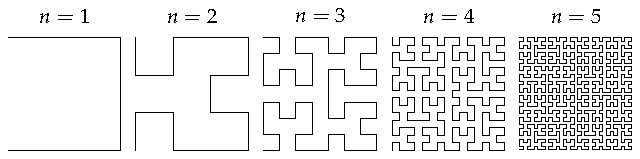
\includegraphics{hilbertcurves.pdf}
%  \checkparity This is an \pageparity\ page.%
  \caption{Curva de Hilbert para diferente $n$.
  \emph{Observa que la figura cubre el ancho del texto}}
  \label{fig:textfig}
\end{figure}

hLorem ipsum dolor sit amet, consectetur adipisicing elit, sed do eiusmod tempor incididunt ut labore et dolore magna aliqua. Ut enim ad minim veniam, quis nostrud exercitation ullamco laboris nisi ut aliquip ex ea commodo consequat. Duis aute irure dolor in reprehenderit in voluptate velit esse cillum dolore eu fugiat nulla pariatur. Excepteur sint occaecat cupidatat non proident, sunt in culpa qui officia deserunt mollit anim id est laborum. hora

\begin{figure*}[h]
  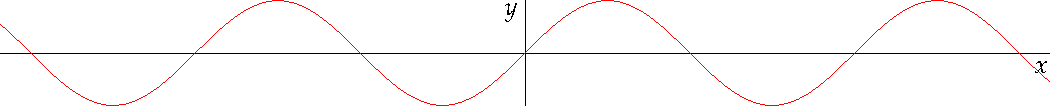
\includegraphics[width=\fullwidthvalue]{sine.pdf}%
  \caption{Con el entorno \texttt{figure*} puedes incluir una figura que cubra el ancho del texto+margen. La variable \texttt{\textbackslash fullwidthvalue} contiene el ancho total del texto. También existe un entorno parecido \texttt{table*} para las tablas.}%
  \label{fig:fullfig}%
\end{figure*}

Lorem ipsum dolor sit amet, consectetur adipisicing elit, sed do eiusmod
tempor incididunt ut labore et dolore magna aliqua. Ut enim ad minim veniam, quis nostrud exercitation ullamco laboris nisi ut aliquip ex ea commodo consequat. Duis aute irure dolor in reprehenderit in voluptate velit esse cillum dolore eu fugiat nulla pariatur. Excepteur sint occaecat cupidatat non proident, sunt in culpa qui officia deserunt mollit anim id est laborum.

\begin{fullwidth}
Puedes incluir párrafos que ocupen el text+margen con el entorno \texttt{fullwidth} como este.

Lorem ipsum dolor sit amet, consectetur adipisicing elit, sed do eiusmod
tempor incididunt ut labore et dolore magna aliqua. Ut enim ad minim veniam, quis nostrud exercitation ullamco laboris nisi ut aliquip ex ea commodo consequat. Duis aute irure dolor in reprehenderit in voluptate velit esse cillum dolore eu fugiat nulla pariatur. Excepteur sint occaecat cupidatat non proident, sunt in culpa qui officia deserunt mollit anim id est laborum.
\end{fullwidth}

Lorem ipsum dolor sit amet, consectetur adipisicing elit, sed do eiusmod tempor incididunt ut labore et dolore magna aliqua. Ut enim ad minim veniam, quis nostrud exercitation ullamco laboris nisi ut aliquip ex ea commodo consequat. Duis aute irure dolor in reprehenderit in voluptate velit esse cillum dolore eu fugiat nulla pariatur. Excepteur sint occaecat cupidatat non proident, sunt in culpa qui officia deserunt mollit anim id est laborum.

\end{document}
